The system shall consist of four main elements: the sensor, the \gls{rpi}, \gls{coap} and the cloud platform.
The sensor will collect the data and pass this to the \gls{rpi}. The \gls{rpi} will then be responsible for manipulating
the data into a suitable format for transmission via \gls{coap}. The implementation of \gls{coap} will communicate with
the cloud platform. The cloud platform will store the data, allowing access to users.

\begin{figure}[H]
    \centering
    \makebox[1\textwidth]{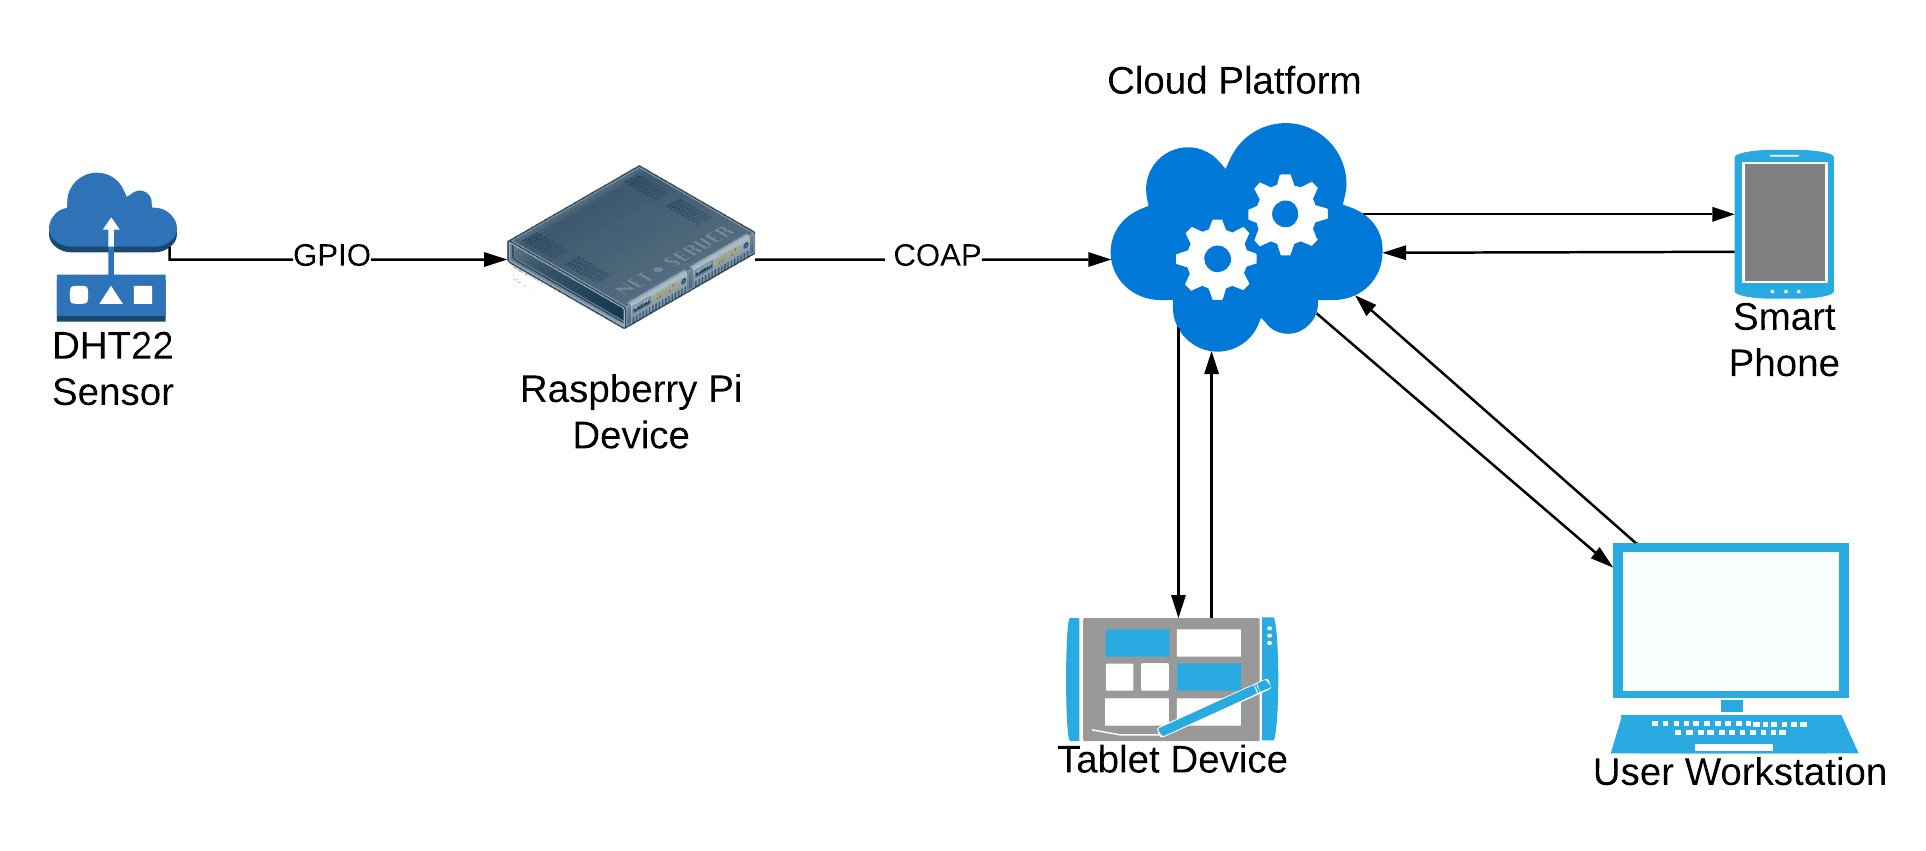
\includegraphics[width=1\textwidth]{assets/Project_Framework.png}}
    \caption{\label{fig:proj_framework} The project infrastructure.}
\end{figure}

The DHT22 sensor will connect to the \gls{rpi} using the \gls{rpi}'s on board \gls{gpio} ports as shown in \figref{fig:rpi_wiring}. 
A Python script using the AdaFruit Python DHT package to retrieve data from the sensor and the CoAPthon Python library will format the sensor data as 
\gls{json}. This script will then make the \gls{json} data available as a \gls{coap} endpoint from which the cloud service can get or subscribe to 
the latest data. 


\begin{figure}[H]
    \centering
    \makebox[1\textwidth]{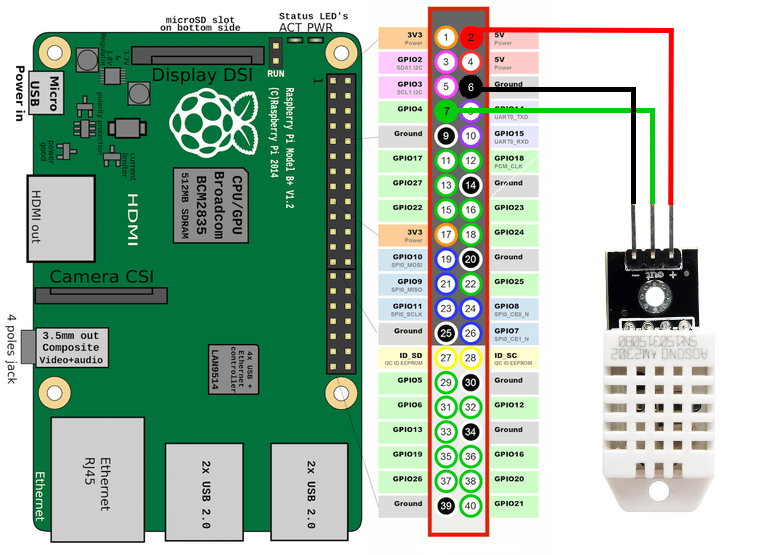
\includegraphics[width=1\textwidth]{assets/rpi_wiring.png}}
    \caption{\label{fig:rpi_wiring} Wiring diagram for connecting the sensor to the \gls{rpi}.}
\end{figure}

\begin{figure}[H]
    \centering
    \makebox[1\textwidth]{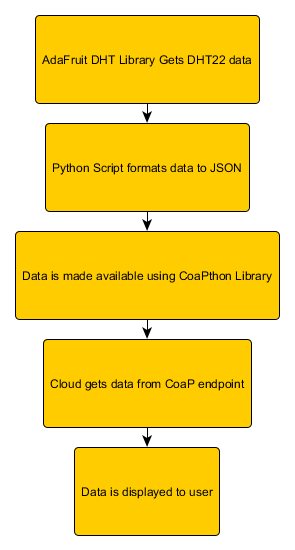
\includegraphics[width=0.5\textwidth]{assets/data_flow.png}}
    \caption{\label{fig:data_flow} Shows the flow of data from sensor to user.}
\end{figure}
